\documentclass[11pt,a4paper]{article}
\usepackage[T1]{fontenc}
\usepackage{lmodern}
\usepackage[margin=22mm]{geometry}
\usepackage{amsmath,amssymb,graphicx,booktabs,microtype}
\usepackage[table]{xcolor}
\usepackage{tikz}
\usepackage{enumitem}
\usepackage{fancyhdr}
\usepackage[colorlinks=true,linkcolor=blue!45!black,urlcolor=blue!45!black]{hyperref}
\definecolor{ink}{HTML}{253047}
\definecolor{muted}{HTML}{667085}
\definecolor{rulegray}{HTML}{DDE2E8}
\setlength{\parindent}{0pt}
\setlength{\parskip}{0.5em}
\setlength{\headheight}{14pt}
\setlist[itemize]{leftmargin=1.3em,itemsep=0.25em,topsep=0.3em}
\setlist[enumerate]{leftmargin=1.5em,itemsep=0.3em,topsep=0.3em}
\pagestyle{fancy}
\fancyhf{}
\fancyhead[L]{\small\color{muted}Rainfall reconstruction: Taylor diagram}
\fancyhead[R]{\small\color{muted}Methodological note}
\fancyfoot[C]{\small\thepage}
\renewcommand{\headrulewidth}{0.3pt}
\hypersetup{pdftitle={A combined Taylor diagram for 100 rainfall patches},pdfsubject={Construction, interpretation, and equal-patch aggregation}}
\newcommand{\avg}[1]{\left\langle #1\right\rangle}
\newcommand{\Var}{\operatorname{Var}}
\newcommand{\Cov}{\operatorname{Cov}}
\newcommand{\Corr}{\operatorname{Corr}}
\begin{document}
\thispagestyle{plain}
{\LARGE\bfseries\color{ink}A combined Taylor diagram\\[0.15em]for 100 rainfall patches\par}
{\color{muted}How to read the figure, why its geometry works, and how patches are combined\par}

We compare six rainfall-reconstruction methods using the saved results for all 100 benchmark patches. Each method is represented by one point summarizing its \textbf{spatial agreement with ground truth}. No solvers were rerun to produce this diagram.

\begin{center}
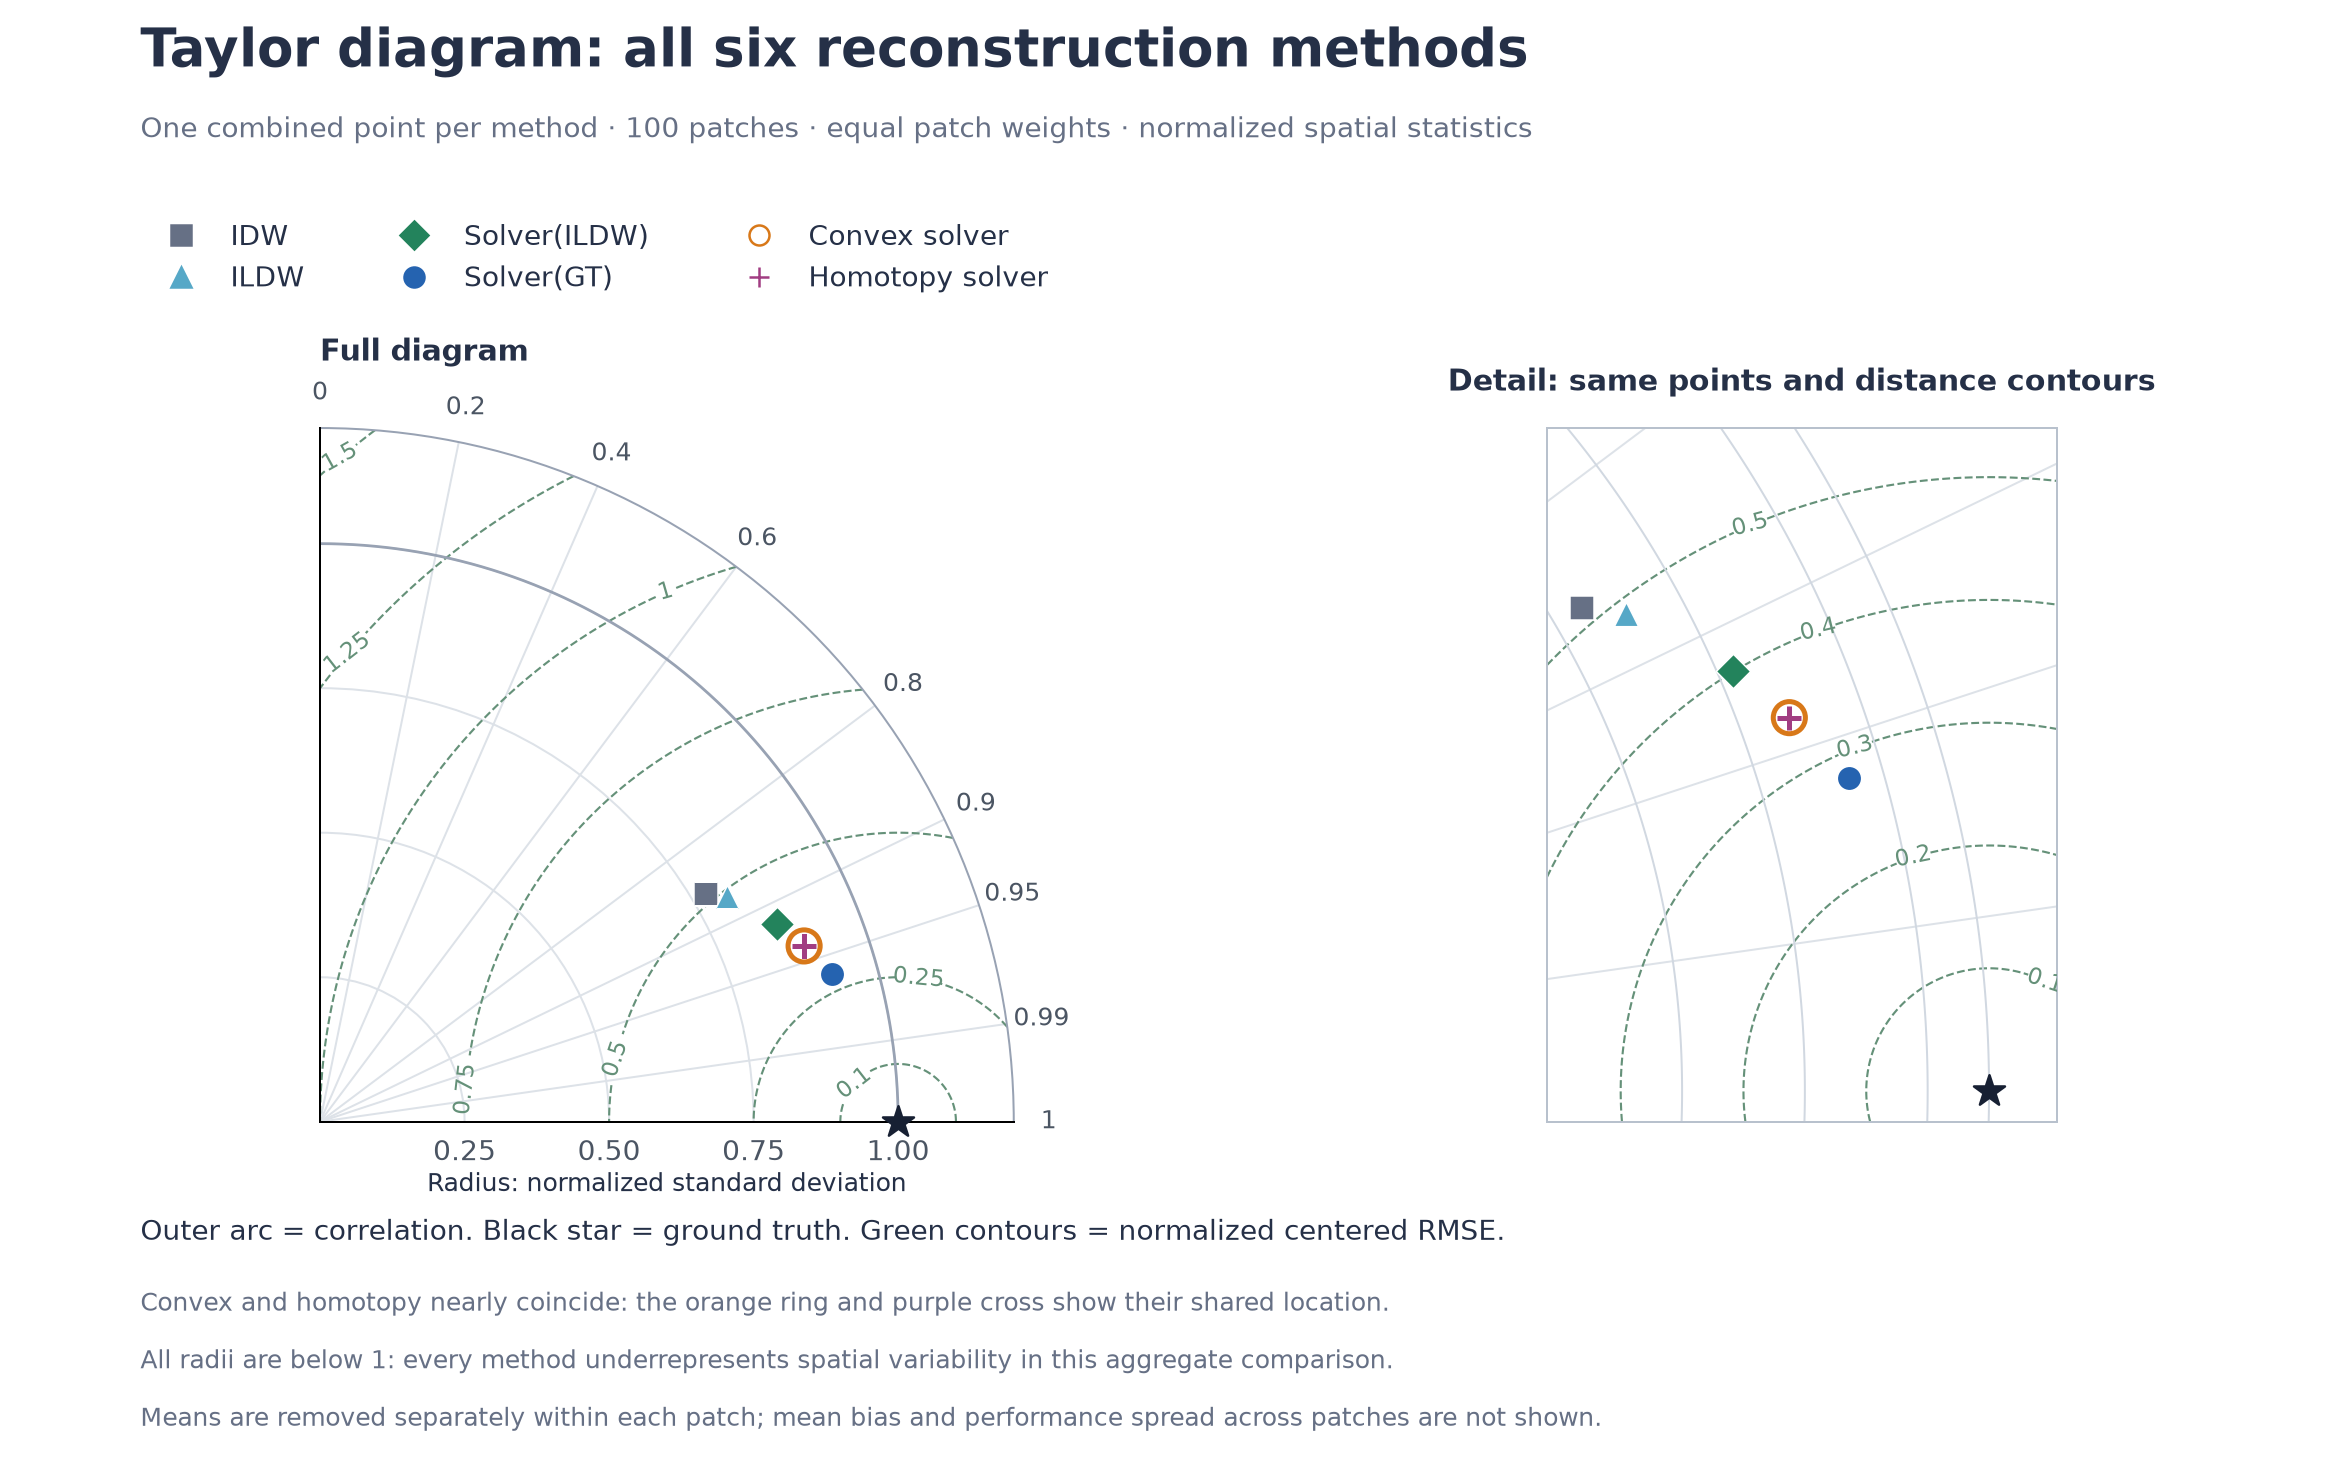
\includegraphics[width=\textwidth]{taylor_all_methods.png}
\end{center}
\vspace{-0.8em}
{\small\textbf{Figure 1.} Normalized Taylor diagram with equal weight per patch. The right panel magnifies the same six points. Distance to the black star measures normalized centered RMSE; the orange ring and purple cross nearly overlap.\par}

{\small In the table, $s_{\mathrm{combined}}$ is the combined standard-deviation \emph{ratio}, $r_{\mathrm{combined}}$ is correlation, and $e_{\mathrm{combined}}$ is normalized centered RMSE. All three are dimensionless.\par}

\begin{center}
\small
\renewcommand{\arraystretch}{1.15}
\begin{tabular}{lrrr}
\toprule
Method & $s_{\mathrm{combined}}$ & $r_{\mathrm{combined}}$ & $e_{\mathrm{combined}}$\\
\midrule
IDW             & 0.776 & 0.862 & 0.514\\
ILDW            & 0.805 & 0.876 & 0.488\\
Solver(ILDW)    & 0.862 & 0.918 & 0.401\\
Solver(GT)      & 0.922 & 0.961 & 0.279\\
Convex solver   & 0.891 & 0.940 & 0.345\\
Homotopy solver & 0.891 & 0.940 & 0.345\\
\bottomrule
\end{tabular}
\end{center}

Solver(GT), which is initialized from the ground-truth field, is closest to the reference. Convex and homotopy have almost identical summary statistics. All six methods have $s_{\mathrm{combined}}<1$, indicating too little spatial rainfall variability under this aggregation. The diagram excludes mean bias and does not show variation in performance between patches.

\newpage
\section*{Start here: what do the symbols mean?}

Fix one reconstruction method. The index $i$ identifies a patch, with $i=1,\ldots,100$. Patch $i$ contains $N_i$ pixels. At pixel $p$, $g_i(p)$ is the ground-truth rainfall and $f_i(p)$ is the rainfall reconstructed by that method. These values are in mm/h.

\textbf{Every method has its own reconstructed field and its own pair $(s_i,r_i)$ for each patch.} We omit a method index to keep the notation readable. All comparisons pair reconstructed and reference values at the same pixel locations.

\subsection*{Standard deviation: variability within one field}
Let $\bar g_i$ and $\bar f_i$ be the pixel averages in the two fields. Their spatial standard deviations are
\[
\sigma_{g_i}=\sqrt{\frac1{N_i}\sum_{p=1}^{N_i}(g_i(p)-\bar g_i)^2},\qquad
\sigma_{f_i}=\sqrt{\frac1{N_i}\sum_{p=1}^{N_i}(f_i(p)-\bar f_i)^2}.
\]
These measure how much rainfall varies between pixels within the patch. Both have units of mm/h. They do not measure variation in performance across the 100 patches.

\subsection*{$s_i$: the standard-deviation ratio}
\[
\boxed{s_i=\frac{\sigma_{f_i}}{\sigma_{g_i}}.}
\]
Thus $s_i$ is \textbf{not the reconstructed standard deviation itself}; it is the reconstructed SD divided by the ground-truth SD. It has no units. A value of 1 means matching spatial variability, below 1 means too little variability, and above 1 means too much.

For example, $\sigma_{g_i}=2$~mm/h and $\sigma_{f_i}=1.6$~mm/h give $s_i=0.8$: the reconstruction has 80\% of the ground truth's spatial standard deviation.

\subsection*{$r_i$: correlation between the two fields}
\[
\boxed{r_i=\Corr(f_i,g_i)=
\frac{\frac1{N_i}\sum_{p=1}^{N_i}(f_i(p)-\bar f_i)(g_i(p)-\bar g_i)}
{\sigma_{f_i}\sigma_{g_i}}.}
\]
This is the \textbf{Pearson correlation across corresponding pixels} of patch $i$. It is a relationship between the reconstruction and ground truth, not a property of the reconstructed field alone. It is dimensionless and lies between $-1$ and 1.

A correlation of 1 means perfect positive linear association, but does not guarantee matching rainfall variability or mean rainfall. For example, $f_i=0.8g_i$ has $r_i=1$ and $s_i=0.8$ when ground truth varies spatially.

\subsection*{From individual patches to one method-level point}
The pairs $(s_i,r_i)$ describe individual patches. The quantities $s_{\mathrm{combined}}$ and $r_{\mathrm{combined}}$ summarize all 100 patches for one method using the construction explained later. The same plotting rules apply to either pair.

\newpage
\section*{Reading the diagram and understanding its geometry}

The black star represents perfect agreement with ground truth in the centered, normalized comparison. A method's position encodes three related quantities:
\begin{itemize}
\item \textbf{Radius:} reconstructed standard deviation divided by ground-truth standard deviation. A radius of 1 means matching spatial variability; a smaller radius means too little variability.
\item \textbf{Angle:} $\theta=\arccos r$, measured from the positive horizontal axis. The outer arc is labelled with $r=\cos\theta$, not with the angle itself.
\item \textbf{Distance to the star:} normalized centered RMSE. The green dashed contours join points with equal error.
\end{itemize}

The standard deviation here measures rainfall variation \emph{between pixels within a field}. It is not an error bar or a measure of how performance varies between patches.

\subsection*{The statistical identity behind the picture}
Consider one patch. Let $g$ and $f$ be its ground-truth and reconstructed pixel values. First subtract each field's own mean:
\[
g'=g-\bar g,\qquad f'=f-\bar f.
\]
Let $\avg{\cdot}$ denote the average over pixels. Standard deviations use the same population convention: $\sigma_g^2=\avg{(g')^2}$ and $\sigma_f^2=\avg{(f')^2}$. Expanding the squared centered error gives
\begin{align*}
E'^2
 &=\avg{(f'-g')^2}\\
 &=\avg{(f')^2}+\avg{(g')^2}-2\avg{f'g'}\\
 &=\sigma_f^2+\sigma_g^2-2r\sigma_f\sigma_g,
\end{align*}
where $r=\Corr(f,g)$, because covariance equals $r\sigma_f\sigma_g$.

This is exactly the form of the \textbf{law of cosines}, $c^2=a^2+b^2-2ab\cos\theta$. A triangle can therefore have sides $\sigma_f$, $\sigma_g$, and $E'$, with angle $\theta=\arccos r$ between its first two sides. This is the basis of the Taylor diagram~\cite{taylor}.

Dividing all lengths by $\sigma_g$ gives the normalized quantities
\[
s=\frac{\sigma_f}{\sigma_g},\qquad e=\frac{E'}{\sigma_g},
\qquad\boxed{e^2=s^2+1-2sr.}
\]
Place the reference at $(1,0)$ and the reconstruction at radius $s$ and angle $\arccos r$. Its distance to the reference is then exactly $e$. Three statistics fit into two dimensions because only two are independent; the identity determines the third.

\subsection*{What centering removes}
The original mean bias $b=\bar f-\bar g$ satisfies $\mathrm{RMSE}^2=E'^2+b^2$. Taylor diagrams show the centered component $E'$, not the bias. A field differing from ground truth only by a constant offset would lie at the reference star, despite its nonzero ordinary RMSE.

\newpage
\section*{Where is the point actually placed?}

The Taylor diagram uses \textbf{polar coordinates}. For either a single patch or a combined summary, let $s$ be the standard-deviation ratio and $r$ the correlation. The plotting instructions are
\[
\boxed{\text{radius}=s,\qquad \theta=\arccos r.}
\]
The angle $\theta$ is measured anticlockwise from the positive horizontal axis. Correlation is not the angle: for example, $r=1$ means $\theta=0^\circ$, while $r=0$ means $\theta=90^\circ$.

\subsection*{Radial distance versus horizontal position}
The corresponding Cartesian coordinates are
\[
\boxed{x=sr,\qquad y=s\sqrt{1-r^2}.}
\]
Consequently, $s$ is the straight-line distance from the origin to the point, not generally its horizontal coordinate. The standard-deviation labels printed along the horizontal axis apply to \emph{circular arcs centered on the origin}; they are a radial scale.

\begin{center}
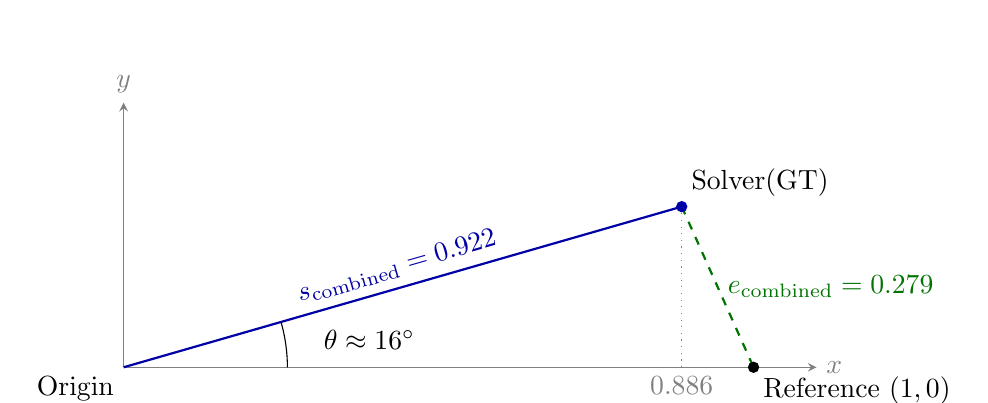
\begin{tikzpicture}[x=8cm,y=8cm,>=stealth]
\draw[->,gray] (0,0)--(1.10,0) node[right] {$x$};
\draw[->,gray] (0,0)--(0,.42) node[above] {$y$};
\draw[thick,blue!65!black] (0,0)--(.886,.255)
 node[midway,above,sloped] {$s_{\mathrm{combined}}=0.922$};
\draw[thick,green!45!black,dashed] (.886,.255)--(1,0)
 node[midway,right] {$e_{\mathrm{combined}}=0.279$};
\draw[dotted,gray] (.886,.255)--(.886,0) node[below] {$0.886$};
\draw (.26,0) arc[start angle=0,end angle=16.05,radius=.26];
\node at (.39,.043) {$\theta\approx16^\circ$};
\fill[blue!65!black] (.886,.255) circle[radius=.009];
\node[above right] at (.886,.255) {Solver(GT)};
\fill (1,0) circle[radius=.009];
\node[below right] at (1,0) {Reference $(1,0)$};
\node[below left] at (0,0) {Origin};
\end{tikzpicture}
\end{center}

\subsection*{Numerical example: Solver(GT)}
Our combined Solver(GT) statistics are $s_{\mathrm{combined}}\approx0.922$ and $r_{\mathrm{combined}}\approx0.961$. The angle is therefore approximately $16^\circ$ and the point is approximately $(0.886,0.255)$. It is 0.922 units from the origin and 0.279 units from the reference. These are different distances with different meanings.

\subsection*{What happens when the angle is zero?}
When $\theta=0$, correlation is 1 and
\[
x=s,\qquad y=0.
\]
\textbf{In this case, radial distance and horizontal position are identical.} The point lies on the positive horizontal axis. It need not coincide with the reference: $s=0.8$ and $r=1$ place it at $(0.8,0)$, with normalized centered RMSE $|1-0.8|=0.2$. Its pattern is perfectly correlated with ground truth, but its variability is too small.

\newpage
\section*{Preparing and combining the 100 patches}

We do not average rainfall maps. We center and normalize each patch separately, then combine its statistical contributions with equal total weight per patch.

For patch $i$, define
\[
u_i=\frac{g_i-\bar g_i}{\sigma_{g_i}},\qquad
v_i=\frac{f_i-\bar f_i}{\sigma_{g_i}}.
\]
Each field uses its \emph{own} mean, but both use the \emph{same ground-truth standard deviation}. Thus the reference SD becomes 1 while the reconstruction retains its relative variability. For example, ground-truth and reconstructed SDs of 2 and 1.6~mm/h become 1 and 0.8. Dividing each field by its own SD would erase that difference.

Writing $s_i=\sigma_{f_i}/\sigma_{g_i}$ and $r_i=\Corr(f_i,g_i)$, we have
\[
\Var(u_i)=1,\qquad \Var(v_i)=s_i^2,\qquad \Cov(u_i,v_i)=s_i r_i.
\]
Because each field is centered, the combined variances and covariance are their patch-level averages. With $K=100$,
\[
\Var(u)=1,\qquad
\Var(v)=\frac1K\sum_i s_i^2,\qquad
\Cov(u,v)=\frac1K\sum_i s_i r_i.
\]
Taking the square root of variance, and dividing covariance by the two standard deviations, gives
\[
\boxed{s_{\mathrm{combined}}=\sqrt{\frac1K\sum_i s_i^2}},
\qquad
\boxed{r_{\mathrm{combined}}=
\frac{\frac1K\sum_i s_i r_i}{s_{\mathrm{combined}}}}.
\]
These are the actual statistics of the combined normalized data, rather than arithmetic averages of the plotted radii and correlations. More explicitly, pixel $p$ in a patch with $N_i$ pixels has weight $1/(KN_i)$, so every patch has total weight $1/K$.

\subsection*{Why the combined point remains a valid Taylor point}
Substituting the combined statistics into the same geometric identity gives
\begin{align*}
e_{\mathrm{combined}}^2
 &=s_{\mathrm{combined}}^2+1
   -2s_{\mathrm{combined}}r_{\mathrm{combined}}\\
 &=\frac1K\sum_i\left(s_i^2+1-2s_i r_i\right)
 =\frac1K\sum_i e_i^2.
\end{align*}
Consequently, \textbf{distance to the reference is the root-mean-square of the patches' normalized centered RMSEs}. It is neither their arithmetic mean nor ordinary RMSE in mm/h. We verified the patch-level identities, the combined identities, and agreement with direct normalized pixel moments for all six methods.

\newpage
\section*{What this summary answers, and what it leaves out}

The aggregation answers the following question:
\begin{quote}
How well does each method reproduce spatial rainfall variations across the benchmark, when every patch receives equal weight and errors are expressed relative to that patch's ground-truth variability?
\end{quote}

\subsection*{Why use this normalization and weighting?}
Normalizing by each patch's ground-truth SD prevents patches with larger rainfall variations from dominating solely because of their physical scale. Equal patch weights also prevent patches with more pixels from automatically contributing more.

This is one evaluation choice. Pooling unnormalized pixels would answer a different question, influenced by rainfall scale and, without compensating weights, patch size. Our formulas follow specifically from centering within patches, ground-truth normalization, and equal patch weights.

The combined correlation is likewise a correlation of the combined normalized fields. It should not be described as the arithmetic mean of the 100 patch correlations.

\subsection*{Information that is compressed or excluded}
\begin{itemize}
\item \textbf{Mean bias is excluded.} Systematic overestimation or underestimation of a patch's mean rainfall must be reported separately.
\item \textbf{Variation between patches is compressed.} A single point cannot show whether a method performs consistently or succeeds on some patches and performs poorly on others.
\item \textbf{Matching points do not imply matching maps.} Two methods can have the same correlation, standard-deviation ratio, and centered RMSE while producing different spatial error patterns. The guaranteed error interpretation is the distance to the reference, not the distance between two method points.
\item \textbf{The summary does not establish the case-study split.} The patch-level scatter plot of convex-solver RMSE against Solver(GT) RMSE retains the individual relative-error comparisons that the combined diagram hides.
\end{itemize}

For the paper, this diagram can provide a compact overall comparison of spatial pattern and variability. Bias statistics and patch-level analyses would supply the complementary information needed to interpret systematic errors and the two case-study regimes.

\textbf{Data checks.} No pixels were excluded. Field shapes and finite values were checked, and all reference and reconstructed SDs were positive. Pixel moments use denominator $N_i$ throughout.

\begin{thebibliography}{9}
\small
\bibitem{taylor}
Taylor, K.~E. (2001).
Summarizing multiple aspects of model performance in a single diagram.
\emph{Journal of Geophysical Research: Atmospheres}, 106(D7), 7183--7192.
\href{https://doi.org/10.1029/2000JD900719}{doi:10.1029/2000JD900719}.
See also the author's
\href{https://pcmdi.llnl.gov/staff/taylor/CV/Taylor_diagram_primer.pdf}{Taylor diagram primer}.
\end{thebibliography}
\end{document}
